\documentclass{article}
\usepackage[utf8]{inputenc}
\usepackage[T1]{fontenc}
\usepackage[]{graphicx}
\usepackage[utf8]{inputenc}
\usepackage{lmodern}
\usepackage[a4paper, margin=1in]{geometry}
\usepackage[english]{babel}
\usepackage{fancyhdr}
\usepackage{minted}

\pagestyle{fancy}
\fancyhf{}
\rhead{Lab Assignment 3}
\lhead{Data Warehousing and Data Mining Lab}
\rfoot{Page \thepage}


\large
\title{C}
\begin{document}
\begin{titlepage}
	\begin{center}
	\vspace{1cm}

	% Titles
	% Information about the University
	{\normalsize \textbf{\textit{Data Warehousing and Data Mining Lab (CSD-421)}} \\ 
	    National Institute of Technology, Hamirpur \par}
		\vspace{1.0cm}
    \line(1,0){400}\\
    [0.65cm]
	\huge{\bfseries DATA WAREHOUSING\\ AND\\ DATA MINING LAB\\(CSD-421)\\LAB ASSIGNMENT 3}\\
	\vspace{1.3cm}
	{\large \textbf { 
	AKSHAT RAJ VANSH (185520)}\par}
	\line(1,0){200}\\
	\vspace{1.0cm}
	\textsc{\LARGE \today}\\
	[1.0cm]     
	
    
    {\includegraphics[scale=1]{nit logo.png}}\\
    \vspace{1.5cm}
    {\normalsize \textbf{\textit{Computer Science Department}} \\ 
	    National Institute of Technology, Hamirpur \par}
    \vspace{0.5cm}
    \end{center}
	
\end{titlepage}
\tableofcontents{}
\clearpage


\section{Program 1}
\subsection{Question}
	{\large \textit { 
Create 500 txt files in a directory. Every file contains 20,000 lines and every line
contain random string of length 20 characters.}\par}
\subsection{Code}
\inputminted[frame=lines,linenos]
{python}{Codes/question1/main.py}
\pagebreak
\subsection{Output}
\begin{center}
    {\Large \textbf{\textit{Question 1 Outputs}}}\\
    \vspace{1.5cm}
    {\includegraphics[scale=.7]{Outputs/question1/output_1.png}}\\
    \vspace{1.5cm}
\end{center}
\pagebreak

\section{Program 2}
\subsection{Question}
	{\large \textit { 
Calculate the execution time to convert all the file to upper case. Save the results
in csv file as given below.}\par}
\subsection{Code}
\inputminted[frame=lines,linenos]
{python}{Codes/question2/main.py}
\subsection{Output}
\begin{center}
    {\Large \textbf{\textit{Question 2 Outputs}}}\\
    \vspace{1.5cm}
    {\includegraphics[scale=.7]{Outputs/question2/output_1.png}}\\
    \vspace{1.5cm}
\end{center}
\pagebreak
\end{document}